\section{Programming concepts}
In high-level programming languages like C and C++, and in \gls{hdl} languages like Verilog, various programming concepts are extensively used. This section describes some concepts that are frequently referred throughout this report.
\subsection{Structures}
A structure, or struct for short, is a complex data-type that can contain multiple variables of varying data-types. This method of packing data, allows for simple transmission of all necessary information about an object between functions.
\subsection{Classes}
A class can contain multiple variables of different data-types, like a struct, but in addition a class can have member-functions and divide its member into a public and a private scope. The private members of a class can only be accessed through public member-functions. This added level of security increase the level of integrity of the objects.
\subsection{Pointers}
A pointer is a variable that is defined to point at a location in memory where another object is stored. The pointer itself contains the memory address of the object it points at.
\subsection{Declaration}
Declaration refers to the process of declaring a type or an object that will be used at a later stage. This can for instance be be a struct in C, a class in C++ or a module in Verilog. A type or an object only needs to be declared once. It can after first definition be used as many times as necessary. An example of a declaration of a struct in C: 
\lstset{language=C++, style=Cstyle}
\begin{lstlisting}
struct Book { char title[128], 
              char author[128], 
              int isbn 
            } ;
\end{lstlisting}
\subsection{Instantiation}
Instantiation is when the object you defined with your declaration, is created and stored at a designated location in memory. When you instantiate an object, you usually assigns it a variable or a name, which is used to refer the object throughout the scope of the object. In Verilog we often talk about module \textit{instantiation}. This is the same concept as in \gls{hll}-languages, but here a declared module is placed inside another module, making it a \textit{sub-module}.
\subsection{Assignment}
Assignment is when you give an instantiated object a value, i.e. you are assigning a value to the object.
\subsection{Defining types}
A user-defined structure or object can be defined as a type in C. The struct-example from above can be defined as a type using the line:
\begin{lstlisting}
typedef struct Book Book_t
\end{lstlisting}
Now an object of the type \textit{struct Book} can be instantiated using the line:

\verb!Book_t mybook!,

where \textit{mybook} is the variable name. Using \textit{typedef} can in many cases save both time and reduce code-size.

\section{Linux tools}
Some tools available in Linux is used throughout the scripts created in this thesis. The following subsections will give a short introduction to the most important tools and its usage.
\subsection{bash}
\textit{bash} is the default shell, or command language interpreter, in Linux. A shell processes macros and executes commands. By adding commands to a file, i.e. a script, a long list of commands can be executed in order. For a script to be executed in the bash shell, the \textit{shebang}-line, the first line of the file, needs to contain the path to the bash shell. The line \verb!#!/bin/bash! can be used in most cases, but for portability, the line \verb!#!/usr/bin/env bash! is the safest choice.

\subsection{make}
\textit{make} is a tool used to decide which parts of a large program needs to be recompiled. The synopsis of \textit{make} is:

\verb!make [OPTIONS] [TARGETS]!

Some options for make are:\\
\verb!-f MAKEFILE     !\textit{Provide the path to the Makefile}
\verb

To use \textit{make}, a \textit{Makefile} describing the relationships between the files of the program is needed. If the Makefile is present in the folder where you run the \textit{make}-tool, you do not need to specify the path to the file. The Makefile can define multiple targets, each performing a separate compilation. There can be dependencies between the targets, forcing the dependency-targets to be compiled before specified target.
\subsection{grep}
\textit{grep} is used to search for the occurrence of a pattern in a given file, and print each line found. The synopsis of \textit{grep} is:

\verb!grep [OPTIONS] PATTERN [FILE...]!

where PATTERN is the pattern to be matched, and FILE is the path to the file(s) to be searched.

Some important options used with \textit{grep} are:\\
\verb!-e PATTERN      !\textit{Provide multiple patterns}\\
\verb!-f FILE         !\textit{Get PATTERN from file}\\
\verb!-c              !\textit{Return number of matched lines}\\
\verb!-m NUM          !\textit{Exit after NUM matches}

If you run the command "\verb!grep "two"!" on a file containing the following lines:

\verb!one two three!\\
\verb!one!\\
\verb!two!

the output will be:

\verb!one two three!\\
\verb!two!

as the first and the last line of the input contains the pattern \textit{two}. More advanced patterns can be described using regular expressions (regex). This allows for matching characters in special positions or order.

\subsection{Substring replacement}

As \textit{grep} returns the whole line that were matched we need a way to eliminate unwanted information from the returned line. For this purpose, the tool \textit{sed} could be used, but when using the \textit{bash}-shell for scripts, a similar tool called \textit{substring replacement} is included natively. The syntax of substring replacement is:

\verb!${string/substring/replacement}!

where \textit{string} is a string, \textit{substring} is the text to be replaced and \textit{replacement} is the string that \textit{substring} will be replaced with. Notice that \textit{string} can be both a literate string and a variable containing a string, depending on the use. This format will only replace the first occurrence of \textit{substring} on each line of \textit{string}. To replace all occurrences, this format must be used:

\verb!${string//substring/replacement}!

If the command "\verb!${"one two one two"//one/three}!" is run, the output would give \verb!"three two three two"!, as all occurrences of the substring \textit{one} will be replaced by \textit{three}.


\begin{figure}
        \centering
        \begin{subfigure}{0.66\textwidth}\centering%no!\hfill
                    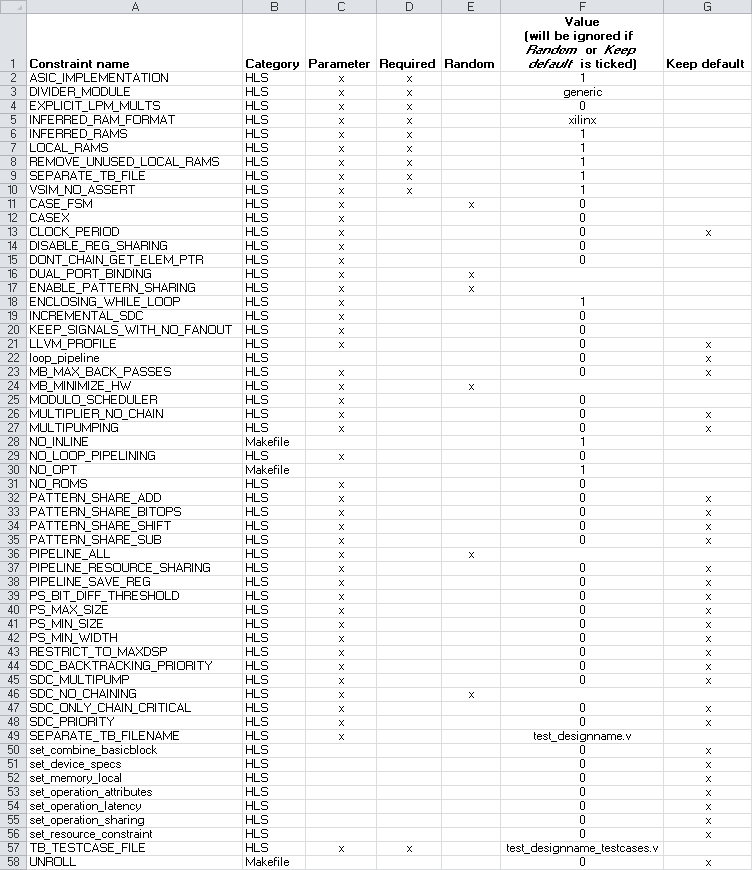
\includegraphics[width=\linewidth]{../figs/ConstraintGenerationSetup.png}
                \caption{Setup page}
  \label{fig:excelconstraintssetup}
       \end{subfigure}%
    \hfill
        \begin{subfigure}{0.32\textwidth}\centering
                    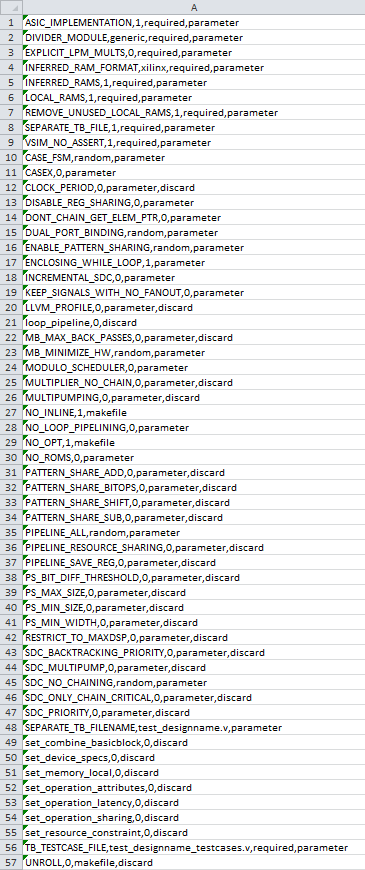
\includegraphics[width=\linewidth]{../figs/ConstraintGenerationCSV.png}
                \caption{CSV format output}
  \label{fig:excelconstraintscsv}
       \end{subfigure}%
    \hfill

\caption{\label{fig:constraintgeneratingexcel}Constraint-file generation in Excel spreadsheet}
 \end{figure}
 